\begin{figure}[t]
\vspace{-10px}
\centering
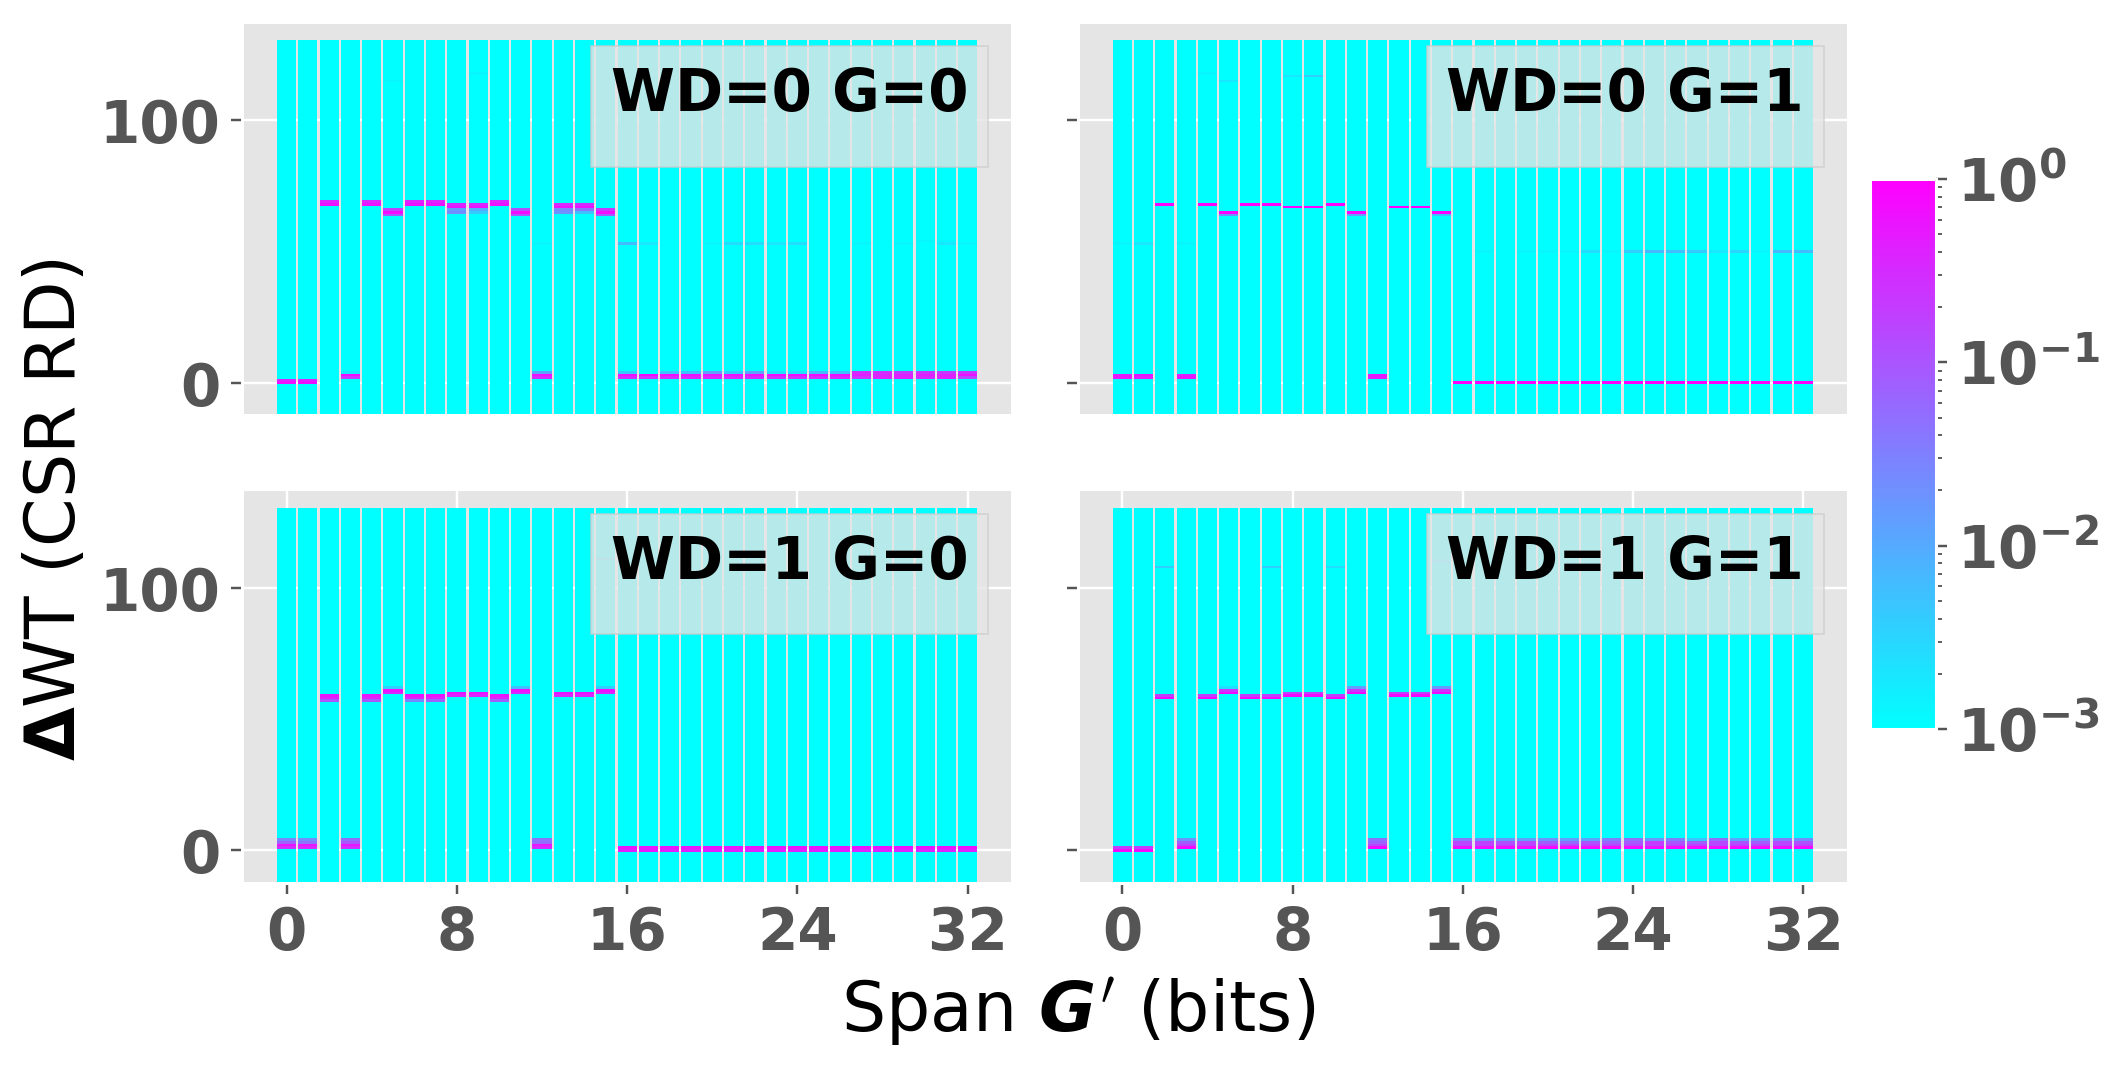
\includegraphics[width=\linewidth]{img/adj_relationship.png}
\caption{Write-time distribution measured while varying the state of logically adjacent memory cells. All write times are measured for a 1-bit transition in a fixed position within a target byte. The global state (G) is the logical state of all bits in the memory at the start of each experiment run. An increasing number of adjacent cells are inverted from G ($G'$) and the transition write-time of the target bit is remeasured. The write data (WD) is the logical state after the switching event used to measure write-time. \label{fig:adj_relationship}}
\end{figure}